

\section{Certification using Noise Injection}
As we will inject some noise in our classifier in order to defend against adversarial attacks, we need to introduce the notion of ``probabilistic mapping''.

\begin{definition}[Probabilistic mapping] Let $\mathcal{X}$ be an arbitrary space, and $(\mathcal{Y},\mathcal{F}_{\mathcal{Y}})$ a measurable space. A \emph{probabilistic mapping} from $\mathcal{X}$ to $\mathcal{Y}$ is a randomized classifier, i.e. a mapping $\probmap: \mathcal{X} \to \mathcal{M}_1^+(\mathcal{Y})$.
To obtain a numerical output out of this \emph{probabilistic mapping}, one needs to sample $y$ according to $\probmap(x)$. %$y\sim \probmap(x)$.
\end{definition} 

Any mapping can be considered as a probabilistic mapping, whether it explicitly injects noise (as in~\citep{lecuyer2018certified,rakin2018parametricnoiseinjection,pruningDefenseICLR2018}) or not. In fact, any deterministic mapping can be considered as a probabilistic mapping, since it can be characterized by a Dirac measure. Accordingly, the definition of a probabilistic mapping is fully general and equally treats networks with or without noise injection. There exists no definition of robustness against adversarial attacks that comply with the notion of probabilistic mappings. We settle that by generalizing the notion of prediction-change risk initially introduced in~\citep{NIPS2018Mahloujifar} for deterministic classifiers. Let $\probmap$ be a probabilistic mapping from $\mathcal{X}$ to $\mathcal{Y}$, and $d_{\mathcal{M}_1^+(\mathcal{Y})}$ some metric/divergence on $\mathcal{M}_1^+(\mathcal{Y})$. We define the $(\varepsilon,\alpha)$-radius prediction-change risk of $\probmap$ w.r.t. $\mathcal{D}_{\mathcal{X}}$ and $d_{\mathcal{M}_1^+(\mathcal{Y})}$ as 
$$\PCadvRisk(\probmap,\alpha):=  \mathbb{P}_{x\sim \mathcal{D}_{\mathcal{X}}}\left[ \exists \tau \in B(\varepsilon) \text{ s.t. } d_{\mathcal{M}_1^+(\mathcal{Y})}(\probmap(x+\tau),\probmap(x)) > \alpha \right] \enspace.$$

These three generalized notions allow us to analyze noise injection defense mechanisms (Theorems~\ref{thm:netrob}, and~\ref{thm:bound}). We can also define adversarial robustness (and later adversarial gap) thanks to these notions. 

\begin{definition}[Adversarial robustness]
\label{def::GeneralizedRobustness}
Let $d_{\mathcal{M}_1^+(\mathcal{Y})}$ be a metric/divergence on $\mathcal{M}_1^+(\mathcal{Y})$. A probabilistic mapping $\probmap$ is called
 $d_{\mathcal{M}_1^+(\mathcal{Y})}$-$(\varepsilon, \alpha, \gamma)$ robust if
$\PCadvRisk(\probmap,\alpha) \leq \gamma$, $d_{\mathcal{M}_1^+(\mathcal{Y})}$-$(\varepsilon, \alpha)$ robust if $\gamma = 0$.
\end{definition}

% \begin{definition}[Adversarial gap]
% \label{def::adversarialgap}
% Let $\probmap$ be a probabilistic mapping from $\mathcal{X}$ to $\mathcal{Y}$. The $\varepsilon$-radius adversarial gap of $\probmap$ is defined as $\text{Gap}_{\varepsilon}(\probmap) = |\advRisk(K) - \Risk(K)|$
% \end{definition}

It is difficult in general to show that a classifier is $d_{\mathcal{M}_1^+(\mathcal{Y})}$-$(\varepsilon, \alpha, \gamma)$ robust. However, we can  derive some bounds for particular divergences that will ensure robustness up to a certain level (Theorem~\ref{thm:netrob}). It is worth noting that our definition of robustness depends
on the considered metric/divergence between probability measures. Lemma~\ref{th::PropimpliesRobustness} gives some insights on the monotony of the robustness according to the parameters, and the probability metric/divergence at hand.

% One needs to be careful when considering adversarial robustness regarding this definition: a robust mapping does not necessarily ensures accuracy. In fact, if $\mathcal{Y}$ is the space of labels $\left[N\right ]$ and $u(x+\tau),u(x)$ respect the same uniform distribution over $\mathcal{Y}$, then for every metric/divergence $d$, one has $d(u(x+\tau),u(x))=0$, and the accuracy will be the one of a random classifier. In the following, \textit{robust} will mean robust in the sense of Definition~\ref{def::GeneralizedRobustness}. Our definition depends on $3$ parameters ($\varepsilon$,$\alpha$,$\gamma$) and on the metric/divergence one chooses to consider between probability measures. Lemma~\ref{th::PropimpliesRobustness} gives some natural insights on the monotony of the robustness according to the parameters, and the probability metric at hand.






%\section{Using Exponential family for adversarial robustness}

%In the following of the paper, we will consider a measurable metric input space $\mathcal{X}$. We denote $\norm{.}_{\mathcal{X}}$ a norm on $\mathcal{X}$ and we suppose the inputs are samples from a distribution $\mathcal{D}$. 




%\subsection{Adversarial attacks problem}
%Let us consider a classification task\footnote{Note that the definition of robustness we provide generalizes to other tasks.} over $\mathcal{X}$. A data $x\in\mathcal{X}$ has a true label $y_{true}\in \left [ N\right ]$. Let  $\hat{f}$ be a trained classifier over $\mathcal{X}$. The problem of generating an adversarial example from an input $x$ writes:

%where $t$ is the target class (with $t\neq \hat{f}(x)$).
%Equation (\ref{attackclassicalproblem}) presents a targeted attack model. For the untargeted attack problem, the condition is changed from $\hat{f}(x+\tau)=t$ to $\hat{f}(x+\tau)\neq \hat{f}(x)$. In this paper, we treat indifferently targeted and untargeted attacks. Figure~\ref{advattack} illustrates the principle of an adversarial attack on $\hat{f}$: a small perturbation $\tau$ applied on an input $x$ fools the classifier. The dashed line represents the boundary decision between two classes. The dashed circle around $x$ represents the maximal amount of noise keeping the adversarial example perceptually close to $x$ (in the case of images). The inputs $x$ and $x+\tau$ looks similar but they are classified with two different labels.


%\begin{figure}[ht]
%\vskip 0.2in
%\begin{center}
%\centerline{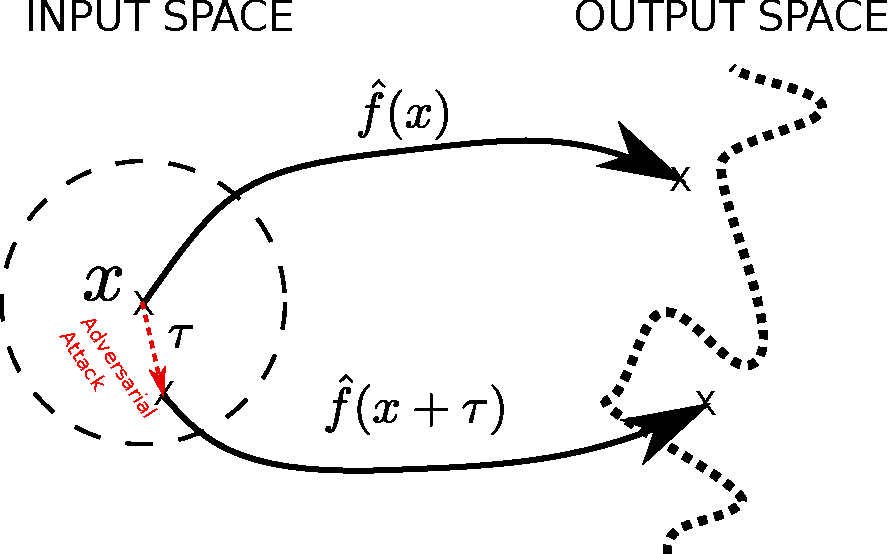
\includegraphics[width=0.5\columnwidth]{images/advAttackV5.pdf}}
%\caption{Illustration of an adversarial attack on a classifier $\hat{f}$. } 
%\label{advattack}
%\end{center}
%\vskip -0.2in
%\end{figure}



%\subsection{A general definition of robustness to adversarial attacks}
%\label{subsec:def}

%As we will inject noise in our algorithm in order to defend against adversarial attacks, we need to introduce the notion of ``probabilistic mapping''. Let us consider $\mathcal{Y}$ the output space, and $\mathcal{F}_{\mathcal{Y}}}$ a $\sigma$-$ algebra$ over $\mathcal{Y}$.

%\begin{definition}[Probabilistic mapping] Let $(\mathcal{Y},\mathcal{F}_{\mathcal{Y}}})$ be a measurable space. For any space $\mathcal{X}$, a \emph{probabilistic mapping} from $\mathcal{X}$ to $\mathcal{Y}$ is a mapping $u: \mathcal{X} \to \mathcal{M}_1^+(\mathcal{Y})$ where $\mathcal{M}_1^+(\mathcal{Y})$ is the set of probability measures over $(\mathcal{Y},\mathcal{F}_{\mathcal{Y}}})$.
%To obtain a numerical output out of this mechanism, one needs to sample $y\sim u(x)$.
%\end{definition} 

% This definition does not depend on the nature of $\mathcal{Y}$ as long as $(\mathcal{Y},\mathcal{F}_{\mathcal{Y}}})$ is measurable. In that sense, $\mathcal{Y}$ could be either the label space $\left[N\right]$ or any  intermediate space corresponding to the outputs of one hidden layer of a neural network. Moreover, any mapping can be considered as a probabilistic mapping, whether it explicitly injects noise (as in~\citep{lecuyer2018certified,rakin2018parametricnoiseinjection,pruningDefenseICLR2018}) or not. In fact, any deterministic mapping can be considered as a probabilistic mapping, since it can be characterized by a Dirac measure. Accordingly, the definition of a probabilistic mapping is fully general and equally treats networks with or without noise injection. So far, there exists no definition of robustness against adversarial attacks that comply with the notion of probabilistic mappings.  We settle that by generalizing the notion of prediction-change risk initially introduced in~\citep{NIPS2018Mahloujifar} for deterministic classifiers. Given a classifier $h$ it is defined as follows:
% $$Risk_\varepsilon(h)= \mathbb{P}_{x\sim \mathcal{D}}\left[ \exists \tau \in B(\varepsilon) \text{ s.t.} h(x+\tau)\neq h(x) \right] $$
% where for any $\varepsilon \geq 0$, $B(\varepsilon) =\{\tau \in \mathcal{X} \text{ s.t.} \norm{\tau}_{\mathcal{X}} \leq \varepsilon \}$. 

% In our case, as probabilistic mappings are considered, we need to generalize this notion to probability measures. This leads to the following definition.
% %Literature on robustness against adversarial examples attacks mostly focuses on the classification setting. Therefore, this work presents a classification task. Our framework could yet adapt to regression, or any other task.



% \begin{definition}[Adversarial robustness]
% \label{def::GeneralizedRobustness}
% Let $d_{\mathcal{M}_1^+(\mathcal{Y})}$ be a metric/divergence on $\mathcal{M}_1^+(\mathcal{Y})$. The probabilistic mapping $u$ is said to be $d_{\mathcal{M}_1^+(\mathcal{Y})}$-$(\varepsilon, \alpha, \gamma)$-robust if:
% $$\mathbb{P}_{x\sim \mathcal{D}}\left[ \exists \tau \in B(\varepsilon) \text{ s.t.} d_{\mathcal{M}_1^+(\mathcal{Y})}(u(x+\tau),u(x)) > \alpha \right] \leq \gamma. $$
% \end{definition}


% Finally, conversely to the previous work, ours does not restrict neither the task (regression, classification, reinforcement learning, etc.) nor the type of distribution the perturbation is drawn from. As $\mathcal{Y}$ is an arbitrary space, this notion of robustness for probabilistic mappings is fully general, but, in this paper, our final goal remains to ensure robustness for a classification task.
% Computing exact divergences and probability measures is unfeasible in practice because neural network functions are too much complicated. But, we can manage to obtain bounds pour divergences that will ensure robustness up to a certain level.

% One needs to be careful when considering adversarial robustness regarding this definition: a robust mapping does not necessarily ensures accuracy. In fact, if $\mathcal{Y}$ is the space of labels $\left[N\right ]$ and $u(x+\tau),u(x)$ respect the same uniform distribution over $\mathcal{Y}$, then for every metric/divergence $d$, one has $d(u(x+\tau),u(x))=0$, and the accuracy will be the one of a random classifier. In the following, \textit{robust} will mean robust in the sense of Definition~\ref{def::GeneralizedRobustness}. Our definition depends on $3$ parameters ($\varepsilon$,$\alpha$,$\gamma$) and on the metric/divergence one chooses to consider between probability measures. Lemma~\ref{th::PropimpliesRobustness} gives some natural insights on the monotony of the robustness according to the parameters, and the probability metric at hand.
% In particular one could consider the deterministic setting by fixing the considered probability measures as Dirac measures, $d_{\mathcal{M}_1^+(\mathcal{Y})}$ as the trivial distance, and $\alpha$ to $0$.
%  In practice, it might be quite hard to evaluate the probability from Definition~\ref{def::GeneralizedRobustness} for any given probabilistic mapping. Nevertheless, as presented in Section~\ref{section::noiseselection}, one should, and can produce algorithms that are robust by design with a noise drawn from an Exponential family.
 
 %In fact one doesn't have access to the ground-truth function, and thus is not able to evaluate $B(\varepsilon)$. Section~\ref{section::noiseselection} will give simple and efficient techniques to comply with the definition, while avoiding to compute this probability.
 


\begin{lemma}
\label{th::PropimpliesRobustness}Let $\probmap$ be a probabilistic mapping, and
let  $d_{1}$ and $d_{2}$ be two metrics on $\mathcal{M}_1^+(\mathcal{Y})$.
If there exists a non decreasing function $ \phi: \mathbb{R} \to \mathbb{R}$ such that  $\forall \mu_1,\mu_2 \in \mathcal{M}_1^+(\mathcal{Y})$, $d_{1}(\mu_1,\mu_2) \leq \phi(d_{2}(\mu_1,\mu_2)) $, then the following assertion holds: 
$\probmap \text{ is } d_{2}\text{-}(\varepsilon, \alpha, \gamma)\text{-robust} \implies \probmap \text{ is }d_{1}\text{-}(\varepsilon, \phi(\alpha), \gamma)\text{-robust}.$
\end{lemma}

As suggested in Definition~\ref{def::GeneralizedRobustness} and Lemma~\ref{th::PropimpliesRobustness}, any given choice of metric/divergence will instantiate a particular notion of adversarial robustness and it should be carefully selected. %The joint goals that should naturally lead to the selection of an appropriate metric/divergence are its coherence with the task at hand, and its strength (we define strength as being able to cover a wide number of other metrics regarding Lemma~\ref{th::PropimpliesRobustness}). 


% \subsubsection{On the choice of the metric/divergence for robustness}
% \label{subsec:div}
% % \Jam{This section needs to be re-organized and simplified. I argue for telling the whole story in a an 'hors d'oeuvre' paragraph before going deeper in the math. To discuss of course. The narration could be as follows, the divergence/metric that generalizes the Bayes risk is the trivial distance with is untractable, but hopefully there is another measure that is related to the Bayes risk is the total variance, which has good properties, however it is still untractable, an hopefully again we have a generalized divergence that provide a rich landscape of behaviors, this one is Renyi...But at the end what we are looking for is a good divergence with goof properties....}

% % \Lau{CHANGED}

% The aforementioned formulation naturally raises the question of the choice of the metric used to defend against adversarial attacks. 
% %At this point, a natural question to be asked is the choice of the metric/divergence we will choose to defend against adversarial attacks. 
% The main notions that govern the selection of an appropriate metric/divergence are  \emph{coherence}, \emph{strength}, and \emph{computational tractability}. A metric/divergence is said to be coherent if it naturally fits the task at hand ({\em e.g.} classification tasks are intrinsically linked to discrete/trivial metrics, conversely to regression tasks). The strength of a metric/divergence refers to its ability to cover (dominate) a wide class of others in the sense of Lemma~\ref{th::PropimpliesRobustness}. 
% In the following, we will focus on both the total variation metric and the Renyi divergence, that we consider as respectively the most coherent with the classification task using probabilistic mappings, and the strongest divergence. We first discuss how total variation metric is \emph{coherent} with randomized classifiers but suffers from computational issues. The Renyi divergence provides good guarantees about adversarial robustness, enjoys nice \emph{computational properties}, in particular when considering  Exponential family distributions, and is \emph{strong} enough to dominate a wide range of metrics/divergences including total variation.

% % \textbf{Dominated measure:} $\mu$ is said to be \emph{dominated} by $\nu$ (denoted $\mu \ll \nu$) if and only if for all $Y \in \mathcal{F}_{\mathcal{Y}}}$, $\ \nu(Y) = 0 \implies \mu(Y)=0$. If $\mu$ is dominated by $\nu$, there is a measurable function $h : \mathcal{Y} \rightarrow [0,+\infty)$ such that for all $Y \in \mathcal{F}_{\mathcal{Y}}}$, $ \mu(Y)=\int_{Y} h \ d\nu$. $ h $ is called the Radon-Nikodym derivative and is denoted $\frac{d \mu}{d \nu}$.

%  Let  $\mu_1$ and $\mu_2$ be two measures in $\mathcal{M}_1^+(\mathcal{Y})$, both dominated by a third measure $\nu$. The trivial distance $ d_{T}(\mu_1,\mu_2):= \mathds{1}\left(\mu_1 \neq \mu_2\right)$ is the simplest distance one can define between $\mu_1$ and $\mu_2$. In the deterministic case, it is straightforward to compute (since the numerical output of the algorithm characterizes its associated measure), but this is not the case in general. In fact one might not have access to the true distribution of the mapping, but just to the numerical outputs. Therefore, one needs to consider more sophisticated metrics/divergences, such as the total variation distance $ d_{TV}(\mu_1,\mu_2):= \sup_{Y \in \mathcal{F}_{\mathcal{Y}}} |\mu_1 (Y) - \mu_2(Y)|.$ The total variation distance is one of the most broadly used probability metrics. It admits several very simple interpretations, and is a very useful tool in many mathematical fields such as probability theory, Bayesian statistics, coupling or transportation theory. In transportation theory, it can be rewritten as the solution of the Monge-Kantorovich problem with the cost function $c(y_1,y_2) =\mathds{1}\left(y_1 \neq y_2\right)$:
% $ \inf\int_{\mathcal{Y}^{2}}\mathds{1}\left(y_1 \neq y_2\right) d\pi(y_1,y_2)\, ,$
% where the infimum is taken over all joint probability measures $\pi$ on $(\mathcal{Y}\times \mathcal{Y}, \mathcal{F}_{\mathcal{Y} } \otimes \mathcal{F}_{\mathcal{Y}})$ with marginals $\mu_1$ and $\mu_2$. According to this interpretation, it seems quite natural to consider the total variation distance as a relaxation of the trivial distance on $[0,1]$ (see~\citep{villani2003topics} for details). In the deterministic case, the total variation and the trivial distance coincides. In general, the total variation allows a finer analysis of the probabilistic mappings than the trivial distance. But it suffers from a high computational complexity. In the following of the paper we will show how to ensure robustness regarding TV distance.

% Finally, denoting by $g_1$ and $g_2$ the respective probability distributions w.r.t. $\nu$,  the Renyi divergence of order $\lambda$~\citep{renyi1961} writes as  $d_{R,\lambda}(\mu_1,\mu_2):=\frac{1}{\lambda -1}\log \int_{\mathcal{Y}} g_2(y)  \left(\frac{g_1(y)}{g_2(y)}\right)^{\lambda} d\nu(y).$
% The Renyi divergence is a generalized measure defined on the interval $(1,\infty)$, where it equals the Kullback-Leibler divergence when $\lambda \rightarrow 1$ (that will be denoted $d_{KL}$), and the maximum divergence when $\lambda \rightarrow \infty$. It also has the very special property of being non decreasing w.r.t. $\lambda$. This divergence is very common in machine learning, especially in its Kullback-Leibler form as it is widely used as the loss function (cross entropy) of classification algorithms. It enjoys the desired properties  since it bounds the TV distance, and is tractable.  Furthermore, Proposition~\ref{prop:RobustTV} proves that Renyi-robustness implies TV-robustness, making it a suitable surrogate for the trivial distance.

\begin{prop}[Renyi implies TV-robustness]
\label{prop:RobustTV}
Let $\probmap$ be a probabilistic mapping, then for all $\lambda\geq1$, $\alpha > 0$, there exists $\alpha' > 0$ s.t. if $\probmap \text{ is }  d_{R,\lambda}\text{-}(\varepsilon, \alpha, \gamma)\text{-robust}$ then $\probmap \text{ is } d_{TV}\text{-}(\varepsilon, \alpha', \gamma)\text{-robust}.$
% $$\textnormal{ with } \alpha' = \min \left(\frac{3}{2}\left(\sqrt{1 + \frac{4\alpha}{9}} - 1\right)^{1/2}, \frac{\exp(\alpha +1) -1}{\exp(\alpha +1) +1}\right) \enspace.$$

%And $\forall\lambda\in(0,1)$:
%$$u \text{ is }  d_{R,\lambda}\text{-}(\varepsilon, \alpha, \gamma)\text{-robust} \implies u \text{ is } d_{TV}\text{-}(\varepsilon,\alpha' , \gamma)\text{-robust} \textnormal{, with } \alpha'=\sqrt{\frac{2\alpha}{\varepsilon}}.$$
\end{prop}

A crucial property of Renyi-robustness is the \textit{Data processing inequality}. It is a well-known inequality from information theory which states that \textit{``post-processing cannot increase information''}~\citep{cover2012elements,beaudry2011intuitive}. In our case, if we consider a Renyi-robust probabilistic mapping, composing it with a deterministic mapping maintains Renyi-robustness with the same level.



\begin{prop}[Data processing inequality]
\label{prop::postprocessing} 
Let us consider a probabilistic mapping $\probmap:\mathcal{X}\rightarrow\mathcal{M}_1^+(\mathcal{Y})$, and denote $\rho:\mathcal{Y}\rightarrow\mathcal{Y}'$ a deterministic function.
If $U\sim \probmap(x)$ then the probability measure $M'(x)$ s.t. $\rho(U) \sim M'(x)$ defines a probabilistic mapping $M':\mathcal{X}\rightarrow\mathcal{M}_1^+(\mathcal{Y}')$. For any $\lambda>1$, if $\probmap$ is $d_{R,\lambda}$-$(\varepsilon,\alpha,\gamma)$ robust then $M'$ is also $d_{R,\lambda}$-$(\varepsilon,\alpha,\gamma)$ robust.
\end{prop}

Data processing inequality will allow us later to inject some additive noise in any layer of a neural network and to ensure Renyi-robustness.

%\section{Noise injection from an Exponential family}
\subsection{Defense mechanisms based on  Exponential family noise injection}
\label{sec:main_result}
\subsubsection{Robustness through Exponential family noise injection}
For now, the question of which class of noise to add is treated \textit{ad hoc}. We choose here to investigate one particular class of noise closely linked to the Renyi divergence, namely Exponential family distributions, and demonstrate their interest.
Let us first recall what the Exponential family is.

\begin{definition}[Exponential family]
Let $\Theta$ be an open convex set of $\mathbb{R}^{n}$, and $\theta \in \Theta$. Let $\nu$ be a measure dominated by $\mu$ (either by the Lebesgue or counting measure), it is said to be part of the \emph{Exponential family} of parameter $\theta$ (denoted $E_{F}(\theta,t,k)$) if it has the following p.d.f.
$$p_{F}(z,\theta)=\exp\left\{ \langle t(z),\theta \rangle -u(\theta) +k(z) \right\} $$
where $t(z)$ is a sufficient statistic, $k$ a carrier measure (either for a Lebesgue or a counting measure) and $u(\theta)= \log \int_{z} \exp\left\{ <t(z),\theta> +k(z) \right\} dz $.

\end{definition}

To show the robustness of randomized networks with noise injected from the Exponential family, one needs to define the notion of sensitivity for a given deterministic function:
\begin{definition}[Sensitivity of a function]
For any $\varepsilon\geq0$ and for any $||.||_A$ and $||.||_B$ two norms, the $\varepsilon$-sensitivity of $f$ w.r.t. $||.||_A$ and $||.||_B$ is defined as $$\Delta^{A,B}_\varepsilon(f):=\sup\limits_{ x,y \in \mathcal{X}, ||x-y||_{A} \leq \varepsilon} ||f(x) - f(y) ||_B \enspace.$$
\end{definition}

Let us consider an  $n$-layer feedforward neural network  $\mathcal{N}(.)=\phi^n\circ...\circ\phi^1(.)$. For any $i\in\left[n\right]$, we define $\mathcal{N}_{|i}(.)=\phi^i\circ...\circ\phi^1(.)$ the neural network truncated at layer $i$. Theorem~\ref{thm:netrob} shows that, injecting noise drawn from an Exponential family distribution ensures robustness to adversarial example attacks in the sense of Definition~\ref{def::GeneralizedRobustness}.







% \begin{thm}[Exponential family ensures robustness]
% \label{thm:netrob}
% Let us denote $\mathcal{N}_{X}^i(.)=\phi^n\circ...\circ\phi^{i+1}(\mathcal{N}_{|i}(.)+X)$ with $X$ a random variable. Then, $\mathcal{N}_{X}^i(.)$ defines a probabilistic mapping that satisfies::




% \begin{itemize}
%     \item If $X\sim E_{F}(\theta,t,k)$  where $t$ and $k$ have non-decreasing modulus of continuity $\omega_t$ and $\omega_k$. Then for any $\varepsilon \geq 0$, $\probmap$ defines a probabilistic mapping that is $d_{R,\lambda}$-$(\varepsilon,\alpha)$ robust with $\alpha = ||\theta||_2 \omega^{B,2}_t(\Delta^{A,B}_{\varepsilon}(\phi)) +\omega_k^{B,1}(\Delta^{A,B}_{\varepsilon}(\phi)) $ where $||.||_2$ is the norm corresponding to the scalar product in the definition of the exponential family density function and $||.||_1$ is here the absolute value on $\mathbb{R}$. The notion of continuity modulus is defined in supplementary material
    
% %Although the Gaussian distribution does not satisfy the modulus of continuity constraint on $t$, we still have robustness for Gaussian noise injection. Let
% \item If $X$ is a centered Gaussian random variable with a non degenerated matrix parameter $\Sigma$. Then for any $\varepsilon \geq 0$, $\probmap$ defines a probabilistic mapping that is $d_{R,\lambda}$-$(\varepsilon,\alpha)$ robust
% with $ \alpha = \frac{\lambda \Delta^{A,2}_{\varepsilon}(\phi)^2 }{2 \sigma_{min}(\Sigma) } $ where $||.||_2$ is the canonical Euclidean norm on $\mathbb{R}^n$.
% \end{itemize}
% \end{theorem}


\begin{thm}[Exponential family ensures robustness]
\label{thm:netrob}
Let us denote $\mathcal{N}_{X}^i(.)=\phi^n\circ...\circ\phi^{i+1}(\mathcal{N}_{|i}(.)+X)$ with $X$ a random variable. Let us also consider two arbitrary norms $||.||_{A}$ and $||.||_{B}$  respectively on $\mathcal{X}$ and on the output space of $\mathcal{N}_{X}^i$.




\begin{itemize}
    \item If $X\sim E_{F}(\theta,t,k)$  where $t$ and $k$ have non-decreasing modulus of continuity $\omega_t$ and $\omega_k$. Then for any $\varepsilon \geq 0$, $\mathcal{N}_{X}^i(.)$ defines a probabilistic mapping that is $d_{R,\lambda}$-$(\varepsilon,\alpha)$ robust with $\alpha = ||\theta||_2 \omega^{B,2}_t(\Delta^{A,B}_{\varepsilon}(\phi)) +\omega_k^{B,1}(\Delta^{A,B}_{\varepsilon}(\phi)) $ where $||.||_2$ is the norm corresponding to the scalar product in the definition of the exponential family density function and $||.||_1$ is the absolute value on $\mathbb{R}$. Notions of continuity modulus is defined in the supplementary material.
    
%Although the Gaussian distribution does not satisfy the modulus of continuity constraint on $t$, we still have robustness for Gaussian noise injection. Let
\item If $X$ is a centered Gaussian random variable with a non degenerated matrix parameter $\Sigma$. Then for any $\varepsilon \geq 0$, $\mathcal{N}_{X}^i(.)$ defines a probabilistic mapping that is $d_{R,\lambda}$-$(\varepsilon,\alpha)$ robust
with $ \alpha = \frac{\lambda \Delta^{A,2}_{\varepsilon}(\phi)^2 }{2 \sigma_{min}(\Sigma) } $ where $||.||_2$ is the canonical Euclidean norm on $\mathbb{R}^n$.
\end{itemize}
\end{thm}

In simpler words, the previous theorem ensures stability in the neural network when injecting noise w.r.t. the distribution of the output. Intuitively, if two inputs are close w.r.t. $\lVert\cdot\rVert_{A}$, the output distributions of the network will be close in the sense of Renyi divergence. It is well known that in the case of deterministic neural networks, the Lipschitz constant becomes bigger as the number of layers increases~\citep{gouk2018regularisation}. By injecting noise at layer $i$, the notion of robustness only depends on the sensitivity of the first $i$ layers of the network and not the following ones. In that sense, randomization provides a more precise control on the ``continuity'' of the neural network. In the next section, we show that thanks to the notion of robustness w.r.t. probabilistic mappings, one can bound the loss of accuracy of a randomized neural network when it is attacked. 

%This generalizes the notion of stability for a deterministic network. But, in that case, the distance between two outputs will depend on the sensitivity of every layers of the networks.  Here we show that the sensitivity level is preserved after injecting noise and independent from the sensitivity of next layers on which the control on the sensitivity is less precise.  %So the predicted labels of two close inputs of the network are ``more likely'' to be the same. The next section will provide bounds on the adversarial risk when the neural network is robust to adversarial attacks in the sense of Renyi divergence. 


%For many usual distributions from Exponential family, the modulus of continuity constraints are not respected. To enforce the respect of these constraints, we might truncate the distribution: if $p(z)$ is the original distribution on a measurable space $\mathcal{Z}$, the underlying truncated distribution on a measurable space $\mathcal{Z'}\in\mathcal{Z}$ is $\Tilde{p}(z)=\frac{p(z)}{K}$ for $z$ in $\mathcal{Z'}$ and where $K$ is a normalization constant. Obviously, $\Tilde{p}$ is still a distribution from Exponential family.

%\textcolor{red}{Let us consider a deterministic feed forward neural network $\mathcal{N}$ with $n$ layers. We denote $\mathcal{N}_{i}$ the corresponding to neural network truncated at layer $i \in [n]$ and $\mathcal{N}_{i|}$ is the network starting at layer $i$ such as $\mathcal{N}=\mathcal{N}_{i|} \circ \mathcal{N}_{i}$. Let consider an input $x$. To obtain a robust probabilistic classifier, we add a noise to layer $i$: $\mathcal{N}_{i}(x)+X$ where $X$ is a random variable from the Exponential family. Then according to Theorems~\ref{prop::postprocessing} and~\ref{thm:exprob}, $\Tilde{\mathcal{N}}(x)=\mathcal{N}_{i|}(\mathcal{N}_{i}(x)+X)$ defines a probabilistic mapping satisfying Renyi-robustness. Figure~\ref{robustness_fig} illustrates our noise injection defense mechanism. $\Tilde{\mathcal{N}}_i(.|\varepsilon_i)$ refers to the perturbed $i$-th layer of networks each respecting $(\varepsilon_i,\alpha,\gamma)$-robustness, for small enough values of $\alpha$, and $\gamma$. $\varepsilon_i$ represents the maximal amount of noise, the probabilistic mapping $\Tilde{\mathcal{N}}_i(.|\varepsilon_i)$ is robust against. It defines a ball (with ray $\varepsilon_i$) on which the outputs of the network are stable. If the amount of injected noise is too small, the $\varepsilon_i$ is smaller than the maximal amount of noise keeping the adversarial example visually close from $x$ (this is the case for $\Tilde{\mathcal{N}}_2(.|\varepsilon_2)$ in Figure~\ref{robustness_fig}). Therefore, the probabilistic mapping is not robust to adversarial attacks. Conversely, when the injected noise is sufficiently big, the outputs of the mapping are stable on a ball that includes the set of adversarial examples (as it is the case for $\Tilde{\mathcal{N}}_1(.|\varepsilon_1)$ in Figure~\ref{robustness_fig}). Thus the probabilistic mapping is robust to adversarial examples. } 
%If the level of to small (the ball of ray $\varepsilon_1$ is smaller than the maximal amount of noise keeping the adversarial example visually close from $x$), the probabilistic mapping is vulnerable to adversarial examples. Conversely, when it is strong 

% \textbf{How is this theorem useful in practice?} Let us consider a deterministic feed forward neural network $\mathcal{N}$ with $n$ layers, where $\mathcal{N}_{i}$ corresponds to the neural network truncated at layer $i \in [n]$. %Let consider an input $x$. 
% To obtain a robust probabilistic classifier, for any input $x$, we add a noise to layer $i$: $\mathcal{N}_{i}(x)+X$ where $X$ is a random variable from the Exponential family. Then according to Theorems~\ref{prop::postprocessing} and~\ref{thm:exprob}, after adding the noise $X$ to the $i$th layer, the whole network defines a probabilistic mapping satisfying Renyi-robustness.

% Figure~\ref{robustness_fig} illustrates our noise injection defense mechanism. $\Tilde{\mathcal{N}}_i(.|\varepsilon)$ refers to the perturbed $i$-th layer of networks each respecting $(\varepsilon,\alpha,\gamma)$-robustness, for small enough values of $\alpha$, and $\gamma$. $\varepsilon$ represents the maximal amount of noise, the probabilistic mapping is robust against. It defines a ball (with radius $\varepsilon$) on which the outputs of the network are stable. Any example falling within the ball defined by $\varepsilon$ will be mapped close to the mapped version of $x$ as shown for $\Tilde{\mathcal{N}}_i(.|\varepsilon_2)$ in Figure~\ref{robustness_fig}. Otherwise, any example out of this ball may be mapped farther (potentially crossing the decision boundary). Depending on the magnitude of $\varepsilon$, the mapping could be made more robust as shown for $\Tilde{\mathcal{N}}_i(.|\varepsilon_1)$ in Figure~\ref{robustness_fig}. To summarize, if the outputs of the mapping are stable on a ball that includes the set of adversarial examples visually imperceptible, the probabilistic mapping will be robust to adversarial examples.

% \begin{figure}[t]
% \vskip 0.2in
% \begin{center}
% \centerline{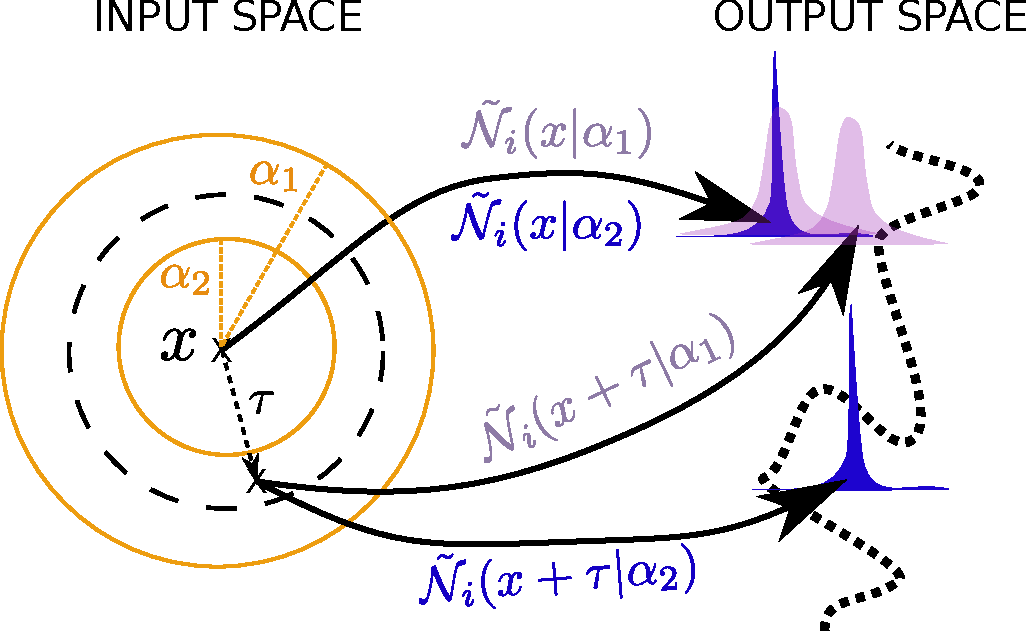
\includegraphics[width=0.5\columnwidth]{images/advAttackRobustV5.pdf}}
% \caption{Illustration of the robustness against adversarial examples for probabilistic mappings (that map images to ditributions).}
% \label{robustness_fig}
% \end{center}
% \vskip -0.2in
% \end{figure}

%$x$ is a natural image and $x+\tau$ an adversarial attack on $x$.  The input space is the space of natural images $\mathcal{X}$, and the output space is the image of $\mathcal{X}$ by the $i$-th layer of the network $\Tilde{\mathcal{N}}_i$. The dashed circle in the input space represents the maximal amount of noise keeping the adversarial example visually close from $x$, and the dashed line in the output space represents the embedding of the decision boundary in the output space of $\mathcal{N}_i$.




% \subsection{On the need for injecting noise in the training phase}
% \label{section::covariateshift}

% So far, we have  designed an algorithm for neural networks to ensure robustness at inference time. But simply injecting noise at inference time destroys the accuracy of the algorithm. Thus one needs to also inject noise during the training phase as well. The justification comes from the distribution shift~\citep{sugiyama2012machine}.
% Distribution shift occurs when the training distribution differs from the test distribution. This implies that the hypothesis minimizing the empirical risk is not consistent, i.e. it does not converge to the true model as the training size increases. A way to circumvent that is to ensure that training and test distributions matches using importance weighting (in the case of covariate-shift) or with noise injection in training and test phases (in our case).
%Let $f$ be the target function one wants to learn, The goal of supervised learning is to approximate this function by a parametrized function $\hat{f}_{\theta}$ from a training dataset $\{(x_i^{tr},y_i^{tr})\}_{i=1}^{n_{tr}}$ i.i.d sampled from an underlying distribution $p_{tr}$. When considering a problem of supervised learning, one assume that the training distribution $p_{tr}$ is actually the same distribution the test distribution $p_{te}$. However, this assumption is not always fulfilled. Situations where training and test datasets follow different distributions are called covariate shift. The interested reader should refer to~\citep{sugiyama2012machine} for a complete introduction on machine learning under covariate shift.
% \Jam{Remove the sequel and put it in the appendice
% The standard method to learn the parameter $\theta$ is the empirical risk minimization (ERM):
% $$\hat{\theta}_{ERM} := \text{argmin}_{\theta}\left[\frac{1}{n_{tr}} \sum_{ i =1}^{n_{tr}} \ell \left(y_i^{tr},\hat{f}_{\theta}\left(x_i^{tr}\right)\right)\right]$$

% where $\ell$ is the loss function at hand.
% The model is said to be correctly specified if there exists a parameter $\theta^{*}$ such that $\hat{f}_{\theta^{*}}=f$. Otherwise, the model is said to be misspecified. It is usually hard to design correctly specified models in machine learning. Hence it is useful to separate models into consistent and non consistent models. 
% A correctly specified model is said to be consistent if $\hat{\theta}_{ERM}$ converges in probability to $\theta^{*}$, as $n_{tr} \rightarrow \infty$. A misspecified model is said to be consistent if it converges to the parameter minimizing the generalization error $$G(\theta) := \mathbb{E}_{(x^{te},y^{te})\sim p_{te}}\left[\ell\left(y^{te},\hat{f}_{\theta}\left(x^{te}\right)\right)\right].$$

% %Since $G(\theta)$ is usually hard to obtain, to evaluate the performance of the obtained model, one can process the empirical generalization error using a test dataset $\{(x_i^{te},y_i^{te})\}_{i=1}^{n_{te}}$ i.i.d sampled from $p_{te}$. 
% %$ G(\theta) = \mathbb{E}_{(X,Y)\sim p_{te}}\left[\ell\left(Y,\hat{f}_{\theta}\left(X\right)\right)\right] $

% If $p_{tr}=p_{te}$, $\hat{\theta}_{ERM}$ is proven to be consistent, but it is not under distribution shift (i.e when $p_{tr}\neq p_{te}$). In fact, ERM remains consistent when the model is correctly specified, but no longer if the model is misspecified . For the sake of readability, for the remaining of this work we denote $\hat{f}:=\hat{f}_{\hat{\theta}_{ERM}}$. 
% }

%\subsection{Bound on the accuracy drop of the method}
\subsubsection{Bound on the risk gap under attack and certified accuracy}

The notions of risk and adversarial risk can easily be generalized to encompass probabilistic mappings. % (e.g by analogy with PAC Bayes theory).

\begin{definition}[Risks for probabilistic mappings]
 Let $\probmap$ be a probabilistic mapping from $\mathcal{X}$ to $\mathcal{Y}$, the risk and the $\varepsilon$-radius adversarial risk of $\probmap$ w.r.t. $\mathcal{D}$ are defined as:
 \begin{align*}
&\risk(\probmap):= \mathbb{E}_{(x,y)\sim \mathcal{D}}\left[ \mathbb{E}_{y'\sim \probmap(x)} \left[ \mathds{1} \left( y' \neq y \right)\right]\right]\\
&\riskadv(\probmap):= \mathbb{E}_{(x,y)\sim \mathcal{D}}\left[ \sup_{\lVert{\tau}\rVert_{\mathcal{X}} \leq \varepsilon}\mathbb{E}_{y'\sim \probmap(x+\tau)} \left[ \mathds{1} \left( y' \neq y \right)\right]\right]\enspace.
\end{align*}
% Regarding the randomization of neural networks, we define the following notions of generalization. For $\Tilde{\mathcal{N}}^i_X$ a randomized neural network with some noise $X$ injected at layer $i$ in:
% \begin{itemize}


%     % \item  Generalization error: $Err(\mathcal{N})=\mathbb{E}_{(x,y)}(1\!\!1_{\mathcal{N}(x)\neq y})$

%     % \item Adversarial generalization error: $Err_\varepsilon(\mathcal{N})=\mathbb{E}_{(x,y)}(\sup_{\tau/\norm{\tau}\leq\varepsilon}1\!\!1_{\mathcal{N}(x+\tau)\neq y})$

%     \item Generalization error for the probabilistic mapping $\Tilde{\mathcal{N}}^i_X$: 
    
%     $$\overline{Err}(\Tilde{\mathcal{N}}^i_X)=\mathbb{E}_{(x,y)}(\mathbb{E}_{X}(1\!\!1_{\Tilde{\mathcal{N}}^i_X(x)\neq y}))$$%=\mathbb{E}_{X}(Err(\Tilde{\mathcal{N}}^i_X))$$
    
%     \item Adversarial generalization error for the probabilistic mapping $\Tilde{\mathcal{N}}^i_X$:
    
%     $$\overline{Err}_\varepsilon(\Tilde{\mathcal{N}}^i_X)=\mathbb{E}_{(x,y)}(\sup_{\tau/\norm{\tau}\leq\varepsilon}\mathbb{E}_{X}(1\!\!1_{\Tilde{\mathcal{N}}^i_X(x+\tau)\neq y}))$$%=\mathbb{E}_{X}(Err_\varepsilon(\Tilde{\mathcal{N}}^i_X))$$
% \end{itemize}

\end{definition}


The definition of adversarial risk for a probabilistic mapping can be matched with the concept of Expectation over Transformation (EoT) attacks~\citep{athalye2018obfuscated}. Indeed, EoT attacks aim at computing the best opponent in expectation for a given random transformation. In the adversarial risk definition, the adversary chooses the perturbation which has the greatest probability to fool the model, which is a stronger objective than the EoT objective. Theorem~\ref{thm:bound} provides a bound on the gap between the adversarial risk and the regular risk:

\begin{thm}[Adversarial risk gap bound in the randomized setting]

\label{thm:bound}
Let $\probmap$ be the probabilistic mapping at hand. Let us suppose that  $\probmap$ is $d_{R,\lambda}$-$(\varepsilon,\alpha)$ robust for some $\lambda\geq1$ then:

$$|\riskadv(\probmap)-\risk(\probmap)|\leq 1-e^{-\alpha}\mathbb{E}_x\left[e^{-H(\probmap(x))}\right]$$
where $H$ is the Shannon entropy $H(p)=-\sum_i p_i \log(p_i)\enspace.$
\end{thm}
This theorem gives a control on the loss of accuracy under attack w.r.t. the robustness parameter $\alpha$ and the entropy of the predictor. It provides a tradeoff between the quantity of noise added in the network and the accuracy under attack. Intuitively, when the noise increases, for any input, the output distribution tends towards the uniform distribution, then, $\alpha\rightarrow0$ and $H(\probmap(x))\rightarrow \log(K)$, and the risk and the adversarial risk both tends to $\frac{1}{K}$ where $K$ is the number of classes in the classification problem. On the opposite, if no noise is injected, for any input, the output distribution is a  Dirac distribution, then, if the prediction for the adversarial example is not the same as for the regular one, $\alpha\rightarrow\infty$ and $H(\probmap(x))\rightarrow 0$. Hence, the noise needs to be designed both to preserve accuracy and robustness to adversarial attacks. In the Section~\ref{section::experiment}, we give an illustration of this bound when $\probmap$ is a neural network with noise injection at input level as presented in Theorem~\ref{thm:netrob}. In practice, we do not have access to the real value of the  entropy, but we estimate it with classical estimators~\citep{paninski2003estimation}.

Our framework being general enough it encompasses several known accuracy certificates from the literature, e.g. the one provided in~\citep{lecuyer2018certified}. Interestingly, we can introduce the following one, based on \emph{our} definition of robustness. 

\begin{thm}
\label{thm::Lecuyerlike}
Let $x \in \mathcal{X}$, and $\probmap$ be a probabilistic mapping with values in $\mathbb{R}^{K}$. If $\probmap$ is $d_{R,\lambda}$-$(\varepsilon,\alpha)$ robust, and if there exist $k^{*}$ and $ \delta^{*} \in (0,1)$ s.t. $\mathbb{E}_{y \sim \probmap(x)}\left[ y_{k^{*}} \right] > e^{2\alpha'} \max\limits_{i \neq k^{*}}\mathbb{E}_{y \sim \probmap(x)}\left[ y_i \right] + (1+ e^{\alpha'})\delta^{*}$, with $\alpha'= \alpha + \frac{\log(1/\delta^{*})}{\lambda - 1}$. Then, for the classifier $ f: x \mapsto \argmaxB\limits_{k \in [K]}\mathbb{E}_{y \sim \probmap(x)}\left[ y_k \right]$ there is no perturbation $\tau \in B(0,\varepsilon)$ such that $f(x)\neq f(x+\tau)$. 
\end{thm}

As the main focus of this work is to give theoretical evidence for randomization techniques, numerical experiments will mainly focus on Theorem~\ref{thm:netrob} and~\ref{thm:bound} and not on certificates (Theorem~\ref{thm::Lecuyerlike}). %illustrating the results from Theorem~\ref{thm:netrob} and Theorem~\ref{thm:bound}.


% \begin{align*}
% |\overline{Err}_\varepsilon(\mathcal{\Tilde{N}}_X^i)-\overline{Err}(\mathcal{\Tilde{N}}_X^i)|  &= |\mathbb{E}_{(x,y)}( \sup_{\tau/\norm{\tau}\leq\varepsilon} \mathbb{E}_X(1\!\!1_{\Tilde{\mathcal{N}}^i_X(x+\tau)\neq y})-  \mathbb{E}_X(1\!\!1_{\Tilde{\mathcal{N}}^i_X(x)\neq y}))| \\
% &=|\mathbb{E}_{(x,y)}( \sup_{\tau/\norm{\tau}\leq\varepsilon} \mathbb{E}_{X_1,X_2}(1\!\!1_{\Tilde{\mathcal{N}}^i_{X_1}(x+\tau)\neq y}-  1\!\!1_{\Tilde{\mathcal{N}}^i_{X_2}(x)\neq y}))|\\
% &\leq\mathbb{E}_{(x,y)}( \sup_{\tau/\norm{\tau}\leq\varepsilon} \mathbb{E}_{X_1,X_2}(|1\!\!1_{\Tilde{\mathcal{N}}^i_X(x+\tau)\neq y}-  1\!\!1_{\Tilde{\mathcal{N}}^i_X(x)\neq y}|))\\
% &=\mathbb{E}_{(x,y)}(\sup_{\tau/\norm{\tau}\leq\varepsilon}\mathbb{P}_{X_1,X_2}(\Tilde{\mathcal{N}}^i_{X_1}(x+\tau)=\Tilde{\mathcal{N}}^i_{X_2}(x)))
% \end{align*}



% where $X_1$ and $X_2$ are two independent samples with the same law than $X$.

% For two discrete random independent variables of law $P=(p_1,...,p_K)$ and $Q=(q_1,...,q_K)$: 
% $$\mathbb{P}(P=Q)=\sum_{i=1}^K p_i q_i \geq \exp{(\sum_{i=1}^K p_i \log q_i)}=\exp{(-d_{KL}(P||Q)-H(P))}$$



\subsection{Numerical experiments}
\label{section::experiment}
To illustrate our theoretical findings, we train randomized neural networks with a simple method which consists in injecting a noise drawn from an Exponential family distribution in the image during training and inference. 
\subsubsection{Experimental setup}
We present our results and analysis on  CIFAR-10, CIFAR-100 \citep{krizhevsky2009learning} and ImageNet datasets \citep{imagenet_cvpr09}. For CIFAR-10 and CIFAR-100 \citep{krizhevsky2009learning}, we used a Wide ResNet architecture \citep{ZagoruykoK16} which is a variant of the ResNet model from \citep{He_2016_CVPR}. We use 28 layers with a widen factor of 10. We train all networks for 200 epochs, a batch size of 400, dropout 0.3 and Leaky Relu activation with a slope on $\mathbb{R}^-$ of 0.1. We minimize the Cross Entropy Loss with Momentum 0.9 and use a piecewise constant learning rate of 0.1, 0.02, 0.004 and 0.00008 after respectively 7500, 15000 and 20000 steps. The networks achieve for CIFAR10 and 100 a TOP-1 accuracy of 95.8\% and 79.1\% respectively on test images. For ImageNet \citep{imagenet_cvpr09}, we use an Inception ResNet v2 \citep{szegedy2017inception} which is the sate of the art architecture for this dataset and achieve a TOP-1 accuracy of 80\%. For the training of ImageNet, we use the same hyper parameters setting as the original implementation. We train the network for 120 epochs with a batch size of 256, dropout 0.8 and Relu as activation function. All evaluations were done with a single crop on the non-blacklisted subset of the validation set.

To transform these classical networks to probabilistic mappings, we inject noise drawn from Laplace and Gaussian distributions, each with various standard deviations. While the noise could theoretically be injected anywhere in the network, we inject the noise on the image for simplicity. More experiments with noise injected in the first layer of the network are presented in the supplementary material. To evaluate our models under attack, we use three powerful iterative attacks with different norms: \emph{ElasticNet} attack (EAD)~\citep{chen2018ead} with $\ell_1$ distortion, \emph{Carlini\&Wagner} attack (C\&W)~\citep{carlini2017towards} with $\ell_2$ distortion and \emph{Projected Gradient Descent} attack (PGD)~\citep{madry2017towards} with $\ell_\infty$ distortion. All standard deviations and attack intensities are in between $-1$ and $1$. Precise descriptions of our numerical experiments and of the attacks used for evaluation are deferred to the supplementary material. 

\textbf{Attacks against randomized defenses:} It has been pointed out by \citep{athalye2017synthesizing,carlini2019evaluating} that in a white box setting, an attacker with a complete knowledge of the system will know the distribution of the noise injected in the network. As such, to create a stronger adversarial example, the attacker can take the expectation of the loss or the logits of the randomized network during the computation of the attack. This technique is called Expectation Over Transformation ($\EoT$) and we use a Monte Carlo method with $80$ simulations to approximate the best perturbation for a randomized network. 

\subsubsection{Experimental results}



\begin{figure}[t]
\centering
\subfigure[]{
    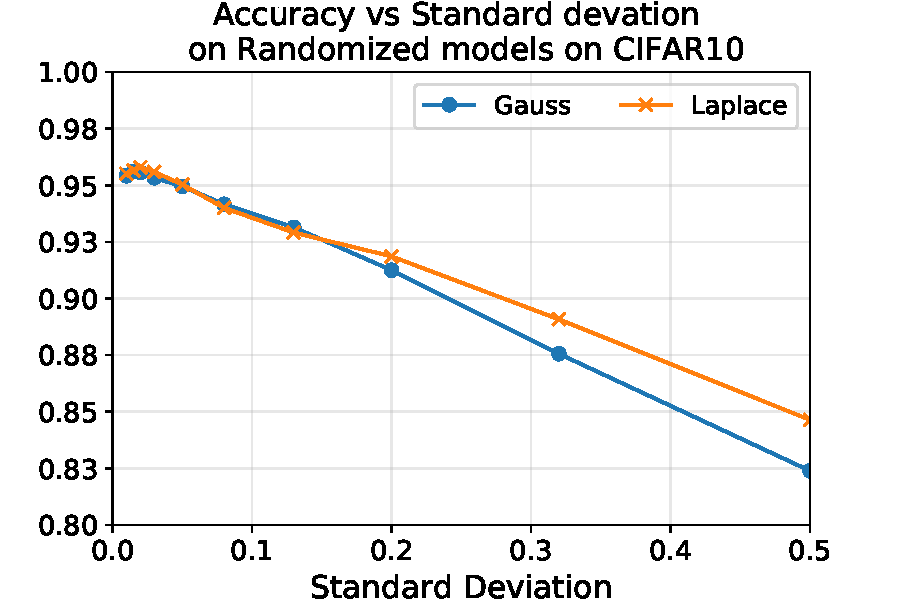
\includegraphics[width=.31\textwidth]{sections/4_certification/images/acc_sd_CIFAR10.pdf}
    \label{fig:acc_sd_CIFAR10}
    }
\subfigure[]{
    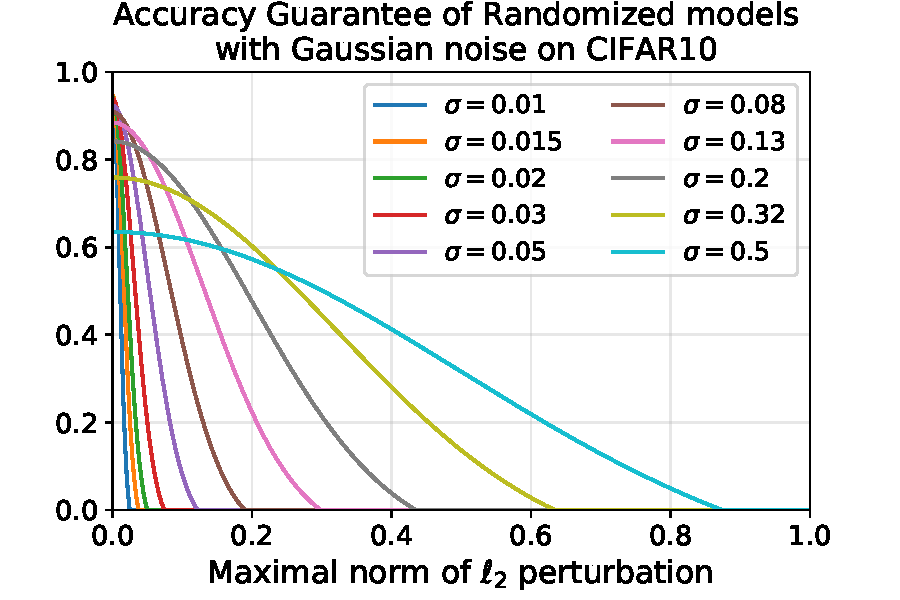
\includegraphics[width=.31\textwidth]{sections/4_certification/images/gauss_certif_CIFAR10.pdf}
    \label{fig:gauss_certif_CIFAR10}
    }
\subfigure[]{
    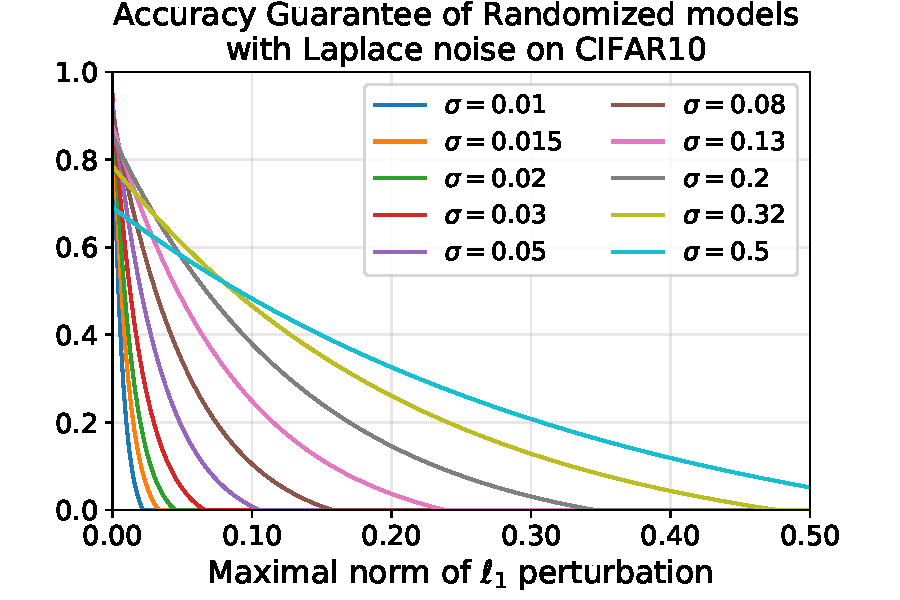
\includegraphics[width=.31\textwidth]{sections/4_certification/images/laplace_certif_CIFAR10.pdf}
    \label{fig:laplace_certif_CIFAR10}
    }
\caption{(a) Impact of the standard deviation of the injected noise on accuracy in a randomized model on CIFAR-10 with a Wide ResNet architecture. (b) and (c) illustration of the guaranteed accuracy of different randomized models with Gaussian (b) and Laplace (c) noises given the norm of the adversarial perturbation. The accuracies and entropies and estimated empirically. \label{fig:cifar10_results}
}
\end{figure}
\textbf{Trade-off between accuracy and intensity of noise:} When injecting noise as a defense mechanism, regardless of the distribution it is drawn from, we observe (as in Figure~\ref{fig:acc_sd_CIFAR10}) that the accuracy decreases when the noise intensity grows. In that sense, noise needs to be calibrated to preserve both accuracy and robustness against adversarial attacks, i.e. it needs to be large enough to preserve robustness and small enough to preserve accuracy. Figure~\ref{fig:acc_sd_CIFAR10} shows the loss of accuracy on CIFAR10 from $0.95$ to $0.82$ (respectively $0.95$ to $0.84$) with noise drawn from a Gaussian distribution (respectively Laplace) with a standard deviation from $0.01$ to $0.5$. Figure~\ref{fig:gauss_certif_CIFAR10} and \ref{fig:laplace_certif_CIFAR10} illustrate the theoretical lower bound on accuracy under attack of Theorem~\ref{thm:bound} for different distributions and standard deviations. The term in entropy of Theorem~\ref{thm:bound} has been estimated using a Monte Carlo method with $10^4$ simulations. The trade-off between accuracy and robustness from Theorem~\ref{thm:bound} thus appears w.r.t the noise intensity. With small noises, the accuracy is high, but the guaranteed accuracy drops fast w.r.t the magnitude of the adversarial perturbation. Conversely, with bigger noises, the accuracy is lower but decreases slowly w.r.t the magnitude of the adversarial perturbation. These Figures also show that Theorem~\ref{thm:bound} gives strong accuracy guarantees against small adversarial perturbations. Next paragraph shows that in practice, randomized networks achieve much higher accuracy under attack than the theoretical bound, and against much larger perturbations.

\textbf{Performance of randomized networks under attacks and comparison to state of the art:}\label{sec:perf_under_attack} While Figure~\ref{fig:gauss_certif_CIFAR10} and \ref{fig:laplace_certif_CIFAR10} illustrated a theoretical robustness against growing adversarial perturbations, Table~\ref{tab:accuracy_under_attack} illustrates this trade-off experimentally. It compares the accuracy under attack of a deterministic network with the one of randomized networks with Gaussian and Laplace noises both with low ($0.01$) and high ($0.5$) standard deviations. Randomized networks with a small noise lead to no loss in accuracy with a small robustness while high noises lead to a higher robustness at the expense of loss of accuracy ($\sim11$ points). Table~\ref{table:madry_vs_random} compares the accuracy and the accuracy under attack of randomized networks with Gaussian and Laplace distributions for different standard deviations against adversarial training~\citep{madry2017towards}. We observe that the accuracy on natural images of both noise injection methods are similar to the one from~\citep{madry2017towards}. Moreover, both methods are more robust than adversarial training to PGD and C\&W attacks. With all the experiments, to construct an $\EoT$ attack,  we use 80 Monte Carlo simulations at every step the attacks. These experiments show that randomized defenses can be competitive given the intensity of noise injected in the network. Note that these experiments have been led with $\EoT$ of size 80. For much bigger sizes of $\EoT$ these results would be mitigated. Nevertheless, the accuracy would never drop under the bounds illustrated in Figure~\ref{fig:cifar10_results}, since Theorem~\ref{thm:bound} gives a bound that on the worst case attack strategy (including $\EoT$).  

\begin{table}[t]
  \centering
  \caption{Accuracy under attack on the CIFAR-10 dataset with a randomized Wide ResNet architecture. We compare the accuracy on natural images and under attack with different noise over 3 iterative attacks (the number of steps is next to the name) made with 80 Monte Carlo simulations to compute EoT attacks. The first line is the baseline, no noise has been injected.}
    \begin{tabular}{lccccc}
    \toprule
    \textbf{Distribution} & \textbf{Sd} & \textbf{Natural} & \textbf{$\ell_1$ -- EAD 60} & \textbf{$\ell_2$ -- C\&W 60} & \textbf{$\ell_\infty$ -- PGD 20} \\
    \midrule
    - & - & 0.958 & 0.035 & 0.034 & 0.384 \\
    \midrule
    \multirow{2}[0]{*}{Normal} & 0.01 & 0.954 & 0.193 & 0.294 & 0.408 \\
          & 0.50 & 0.824 & 0.448 & 0.523 & 0.587 \\
    \midrule
    \multirow{2}[0]{*}{Laplace} & 0.01 & 0.955 & 0.208 & 0.313 & 0.389 \\
          & 0.50 & 0.846 & 0.464 & 0.494 & 0.589 \\
    \bottomrule
    \end{tabular}%
  \label{tab:accuracy_under_attack}%
\end{table}%



% \subsection{Comparison with Adversarial Training (Q4)}\label{sec:adv_madry}

\begin{table}[t]
  \caption{Accuracy under attack of randomized neural network with different distributions and standard deviations versus adversarial training by Madry et al. \citep{madry2017towards}. The PGD attack has been made with 20 step, an epsilon of 0.06 and a step size of 0.006 (input space between $-1$ and $+1$). The Carlini\&Wagner attack uses 30 steps, 9 binary search steps and a 0.01 learning rate. The first line refers to the baseline without attack.}
  \label{Results}
  \centering
  \begin{tabular}{ccccccc}
    \toprule
      & & \multirow{2}[0]{*}{\citep{madry2017towards}} & \multirow{2}[0]{*}{\textbf{Normal 0.32}} & \multirow{2}[0]{*}{\textbf{Laplace 0.32}} & \multirow{2}[0]{*}{\textbf{Normal 0.5}} & \multirow{2}[0]{*}{\textbf{Laplace 0.5}} \\
     \textbf{Attack} & \textbf{Steps} & & & \\
    \midrule
    -  & - & 0.873 & 0.876 & 0.891 & 0.824 & 0.846 \\ 
    $\ell_\infty$ -- PGD & 20 & 0.456 & 0.566 & 0.576 & 0.587 & 0.589 \\
    $\ell_2$ -- C\&W & 30 & 0.468 & 0.512 & 0.502 & 0.489 & 0.479 \\
    \bottomrule
  \end{tabular}
  \label{table:madry_vs_random}
\end{table}


% \subsection{Conclusion and future work}
% \label{section::conclusion}
% This paper brings new contributions to the field of provable defenses to adversarial attacks. Principled answers have been provided to key questions on the interest of randomization techniques, and on their loss of accuracy under attack. The obtained bounds have been illustrated in practice by conducting thorough experiments on baseline datasets such as CIFAR and ImageNet. We show in particular that a simple method based on injecting noise drawn from the Exponential family is competitive compared to baseline approaches while leading to provable guarantees. Future work will focus on investigating other noise distributions belonging or not to the Exponential family, combining randomization with more sophisticated defenses and on devising new tight bounds on the adversarial risk gap.

% \textbf{Acknowledgements: }  This work was granted access to the OpenPOWER prototype from GENCI-IDRIS under the Preparatory Access AP010610510 made by GENCI. R. Pinot benefited from a JSPS Summer Program Fellowship during this work (Grant number SP18218). L. Meunier and J. Atif would also like to thank Adrien Balp from Société Générale for his support.

%Our work contributes to the body of work on defense strategies through randomization by answering key questions on the interest of the Exponential family as a noise generating family and on the adversarial generalization gap bound for associated randomized networks. The bounds are only effective on low dimensional images/limited size perturbations because the ratio between an adversarial perturbation norm and the standard deviation of the injected noise increases as the dimension grows. However, the experimental results are encouraging on every datasets (including ImageNet). Future work will focus on investigating other noise families, combining randomization with more involved defenses and on devising new tight bounds on the adversarial generalization gap. 

% %Injecting noise drawn from an Exponential family in a neural network  has proved its efficiency both from theoretical and experimental standpoints. 
% Our work contributes to the body of work on defense strategies through randomization by answering key questions on the interest of the Exponential family as a noise generating family and on the adversarial generalization gap bound for associated randomized networks.  
% %randomized networks~\citep{lecuyer2018certified,KolterRandomizedSmoothing} that propose a certificate, by presenting a guarantee on the drop of accuracy under attacks for $\ell_2$  or $\ell_1$ norms. It also provides principled arguments supporting the use of randomization as a defense technique.  
% But so far, as for former works, the provided guarantees only hold for small size perturbations. Moreover, the theoretical bounds are only effective on low dimensional images as CIFAR because the ratio between an adversarial perturbation norm and the noise standard deviation of the injected noise rapidly increases as the dimension grows. However, the experimental results are encouraging on every dataset including ImageNet. %It has also been shown that these methods also present a trade-off between accuracy and adversarial robustness. 
% Future work will focus on investigating other noise families, belonging to or beyond the Exponential family, combining the randomization technique with more involved defenses (e.g. adversarial training, ensembles, etc.) and on devising new tight bounds on the adversarial gap. 

%Most empirical defenses against adversarial attacks have been defeated~\citep{athalye2018obfuscated}. Compared to these methods, randomized networks have the advantage to provide theoretical guarantees and to be independent from the neural architecture of the networks. Randomized techniques also experimentally scale well to higher dimension inputs and seem to provide equivalent or better results than classical adversarial training. In future work, we plan to investigate more complex architectures, other noise injection schemes and even the combination with other defenses~\citep{madry2018towards,goodfellow2014explaining}. But more importantly, we aim at developing new family of noise (respecting conditions of Theorem~\ref{thm:netrob}) further impeding the loss of accuracy.

%This is a cool paper

% % donner un cadre theotrique pour comprendre pourquoi les methodes prec d'injection de bruit
% In this work, we bring a theoretically well-grounded framework in order to understand why previous methods based on noise injection were in practice effective against adversarial attacks.  While the very article is a theoretical analysis, it also paves the way to novel defense mechanisms using noises from yet unexplored distributions.
% %In this work, we propose a theoretical insight on why randomizing neural networks makes them more robust against adversarial attacks. We provide a simple methodology that ensures the classifier to be robust. We have proved the wide class of Exponential family distributions can be used to defend against adversarial attacks.

% Our theoretical analysis mainly focused on the robustness of the methods but our numerical experiments validated that the accuracy was slightly altered by noise injection. Hence, we demonstrated the practical applicability of the approach. Note also that as we only used a vanilla ResNet21, using tricks of the trade for neural networks and the noise injection, the accuracy could be further improved.
% %We provided experiments to support our results and we clearly improve robustness by injecting noise at a layer in a feed forward neural network. However, there still exists a trade off between the noise intensity and the accuracy: adding noise increases robustness against adversarial attacks but weakens the accuracy of the classifier. But so far, even a small intensity noise helps defending against adversarial attacks without loosing a lot of accuracy. 

% In future work, we plan to investigate more complex architectures, other noise injection schemes and even the combination with other defenses~\citep{madry2018towards,goodfellow2014explaining}. But more importantly, we aim at developing new family of noise (respecting conditions of Theorem~\ref{thm:netrob}) further impeding the loss of accuracy.

